\documentclass[12pt,prb,aps]{revtex4-1}
\usepackage {amsmath}
\pdfoutput = 1 
\usepackage {graphicx}
\newcommand {\bomega}{\mbox{\boldmath$\omega$}}
\newcommand {\bpi}{\mbox{\boldmath$\pi$}}

\begin{document}

\title {Further Modeling of $q_{95}$ Windows for the Suppression of Edge Localized Modes by Resonant Magnetic Perturbations in the DIII-D Tokamak}

\author{R.~Fitzpatrick\,\footnote{rfitzp@farside.ph.utexas.edu}}
\affiliation{Institute for Fusion Studies,  Department of Physics,  University of Texas at Austin,  Austin TX, 78712, USA}

\begin{abstract}
An improved resonant plasma response model that describes the interaction between a tokamak plasma and a resonant magnetic perturbation  (RMP) is developed. 
The model interpolates between the linear and the nonlinear response regimes, and takes into account the fact that the slip-frequency
is non-zero in the nonlinear regime. The improved model is incorporated into the {\tt EPEC} toroidal asymptotic matching code.
The modified {\tt EPEC} code is used to investigate RMP-induced edge-localized-mode (ELM) mitigation/suppression in DIII-D H-mode discharge \#145380. 
Allowing for a finite slip-frequency (i.e., relaxing the so-called no-slip constraint) is found to slightly facilitate the locking of
driven magnetic island chains to the RMP, and, hence, to slightly facilitate RMP-induced ELM mitigation/suppression.  The previously obtained conclusion 
that the response of a typical H-mode tokamak plasma to an RMP cannot be accurately modeled by linear theory is confirmed. The previously obtained conclusion that the best agreement between theory and observations is achieved by assuming that the
natural frequencies of tearing modes, in the absence of the RMP, are determined by the local equilibrium ${\bf E}\times{\bf B}$ frequency is also confirmed.
\end{abstract}

\maketitle

\section{Introduction}
In the context of tokamak plasmas, a resonant magnetic perturbation (RMP) refers to an externally
generated, (usually) static, helical magnetic perturbation that resonates at
one or more ``rational'' magnetic flux-surfaces within the plasma. Resonant magnetic perturbations have been successfully
employed to compensate error fields (i.e., accidentally produced RMPs), and, thereby,  to prevent the associated formation of
locked modes, in a wide variety of different types of tokamak discharge. \cite{error1,error2,error3} RMPs have also been  successfully used to either  
mitigate or completely suppress  edge-localized-modes (ELMs) in H-mode tokamak discharges.\cite{elm1,elm2,elm3,elm4,elm5,elm6}

``Asymptotic matching'' is by far the most efficient method for modeling the response of a tokamak plasma to an RMP.\cite{fkr,coppi,ruth,ara,pletz,rfa, am1,tokuda,brennan,am2,am3} 
According to the asymptotic matching approach, the response of the plasma to the applied RMP is governed by a combination of flux-freezing and
perturbed force balance---this combination is usually referred to as ``marginally-stable ideal-magnetohydrodynamics (MHD)"---everywhere in the plasma apart from a number of relatively narrow (in the radial direction) regions in which the applied
perturbation resonates with the equilibrium magnetic field. Magnetic reconnection can take place within the resonant regions to
produce relatively narrow magnetic island chains. Within the resonant regions, the plasma response is governed by  linear or nonlinear 
 two-fluid resistive-MHD, depending on whether the induced magnetic island widths are smaller or larger, respectively, than the corresponding linear layer widths. 
 Thus, when employing the asymptotic matching approach, the equations of marginally-stable ideal-MHD
are solved in the so-called ``outer region'' that comprises most of the plasma (and the surrounding vacuum), the equations of 
linear/nonlinear two-fluid resistive-MHD are solved in the various resonant layers that constitute the so-called ``inner region'', and the two
sets of solutions are then asymptotically matched to one another. 

In the nonlinear resonant response regime, the evolution of the island chain width in a given resonant layer is governed by the familiar ``Rutherford island width evolution equation''.\cite{ruth,ruth1}
On the other hand, the phase evolution of the island chain is conventionally governed by the well-known ``no-slip constraint''.\cite{rfa} According to this constraint,  plasma is trapped inside the
magnetic separatrix of the island chain,
which forces the chain to co-rotate with the local plasma flow. In reality, however, the plasma
is able to diffuse resistively across the separatrix to some extent.\cite{slip1,slip2} 

The recently developed, toroidal, asymptotic matching code {\tt EPEC} (Extended Perturbed Equilibrium Code) has been used to simulate 
RMP-induced ELM mitigation/suppression in DIII-D H-mode plasmas.\cite{rftor,rftor1}
The original {\tt EPEC} model incorporates the no-slip constraint.
The first aim of this paper is to investigate 
what happens when the no-slip constraint is relaxed in the aforementioned {\tt EPEC} simulations.
 The second aim is to examine what happens when an improvement is made to the manner in which the resonant
plasma response component of the {\tt EPEC} model interpolates between the linear and the nonlinear regimes. 

\section{Cylindrical Resonant Response Model}\label{s2}
\subsection{Introduction}
For the sake of simplicity, and also to make a better connection with previous research, let us commence our investigation by discussing
the resonant response of a tokamak plasma to an RMP in cylindrical geometry. 

\subsection{Plasma Equilibrium}
Consider a large aspect-ratio, low-$\beta$, tokamak plasma whose magnetic flux-surfaces map out (almost)
concentric circles in the poloidal plane.
Such a plasma is well approximated as a periodic cylinder.  Suppose that the minor radius of the plasma
is $a$. Standard cylindrical coordinates ($r$, $\theta$, $z$) are adopted. The system is assumed to
be periodic in the $z$-direction, with periodicity length $2\pi\,R_0$, where $R_0\gg a$ is the simulated
plasma major radius. It is convenient to define the simulated toroidal angle $\phi=z/R_0$. 

The equilibrium magnetic field is written ${\bf B} = [0,B_\theta(r), B_\phi]$. The associated equilibrium
plasma current density takes the form ${\bf j} =[0,0,j_\phi(r)]$, where $\mu_0\,j_\phi= (1/r)\,d(r\,B_\theta)/dr$. The
so-called ``safety-factor'', $q(r)=r\,B_\phi/(R_0\,B_\theta)$, parameterizes the helical pitches of equilibrium magnetic
field-lines. 

\subsection{Plasma Response to RMP}
Consider the response of the plasma to an externally generated, static, helical, RMP. 
Suppose that the RMP has $m$ periods in the poloidal direction, and $n$ periods in the toroidal direction.
It is convenient to express the perturbed magnetic field and the perturbed plasma current density in
terms of a perturbed poloidal magnetic flux (divided by $2\pi\,R_0$), $\psi(r,\theta,\phi,t)$. In fact, $\delta{\bf B} = \nabla\psi\times \nabla z$, 
and $\mu_0\,\delta {\bf j} = - \nabla^2\psi\,\nabla z$,
where $\psi(r,\theta,\phi,t) = \hat{\psi}(r,t)\,\exp[{\rm i}\,(m\,\theta-n\,\phi)]$, and $\hat{\psi}$ is real. This particular representation
is valid provided that $m/n\gg a/R_0$.\cite{rfa}

The response of the plasma to the RMP is governed by the equations of marginally-stable, ideal-MHD everywhere in the
plasma, apart from a relatively narrow (in $r$) region in the vicinity of the so-called  ``rational surface'', minor radius $r_s$, 
at which $q(r_s)=m/n$.\cite{rfa}

It is convenient to parameterize the RMP in terms of the so-called ``vacuum magnetic flux'', ${\mit\Psi}_v(t) = |{\mit\Psi}_v|\,{\rm e}^{-{\rm i}\,\varphi_v}$,
which is defined to be the value of $\hat{\psi}(r,t)$ at radius $r_s$ in the presence of the RMP, but in the absence of plasma. Here,
$\varphi_v$ is the helical phase of the RMP. Likewise, the response of the plasma in the vicinity of the rational
surface is parameterized in terms of the so-called ``reconnected magnetic flux'', ${\mit\Psi}_s(t)=|{\mit\Psi}_s|\,{\rm e}^{\,{\rm i}\,\varphi_s}$, 
which is the actual value of $\hat{\psi}(r,t)$ at radius $r_s$. Here, $\varphi_s$ is the helical phase of
the reconnected magnetic flux.

The intrinsic stability of the $m$, $n$ tearing mode is governed by the dimensionless parameter
$E_{ss}= [d\hat{\psi}_s/d\ln r]_{r_{s-}}^{r_{s+}}$, where $\hat{\psi}_s(r)$
is a solution of the marginally-stable, ideal-MHD equations, for the case of an $m$, $n$ helical
perturbation, that satisfies physical boundary conditions at $r=0$ and $r=a$, in the absence of the
RMP, and is such that $\hat{\psi}_s(r_s)=1$.\cite{fkr,am1} According to resistive-MHD theory,\cite{fkr,ruth}
if $E_{ss}>0$ then the $m$, $n$ tearing mode spontaneously reconnects magnetic flux at the rational
surface to form a helical magnetic island chain. In this paper, it is assumed that $E_{ss}<0$, so that the
$m$, $n$ tearing mode is intrinsically stable. In this case, any magnetic reconnection that takes place
at the rational surface is due solely to the action of the RMP.

The ideal-MHD response of the plasma to the RMP is governed by the dimensionless parameter
$E_{sv}= [d\hat{\psi}_v/d\ln r]_{r_{s-}}^{r_{s+}}$, where $\hat{\psi}_v(r)$
is a solution of the marginally-stable, ideal-MHD equations, for the case of an $m$, $n$ helical
perturbation, that satisfies physical boundary conditions at $r=0$ and $r=a$, in the presence of the
RMP, and is such that $\hat{\psi}_v(r_s)=0$.\cite{am1} 

\subsection{Linear Response Regime}
In the linear response regime, the reconnected magnetic flux induced by the RMP at the
rational surface is governed by\,\cite{rfa,rfb,rfc}
\begin{equation}\label{e1}
\frac{\delta_s}{r_s}\,\tau_R\left(\frac{d}{dt}+{\rm i}\,\omega_s\right){\mit\Psi}_s= E_{ss}\,{\mit\Psi}_s+E_{sv}\,{\mit\Psi}_v,
\end{equation}
where $\delta_s$ is the linear layer width, $\tau_R=\mu_0\,r_s^{\,2}\,\sigma(r_s)$ the global resistive diffusion timescale,
 and
\begin{equation}
\omega_s (t)=m\,{\mit\Omega}_\theta(r_s,t)-n\,{\mit\Omega}_\phi(r_s,t).
\end{equation}
Here, $\sigma(r)$, ${\mit\Omega}_\theta(r,t)$, and ${\mit\Omega}_\phi(r,t)$ are the 
plasma electrical conductivity, poloidal angular velocity, and toroidal angular velocity profiles, respectively. 
Note that, in this paper, we are assuming that the constant-$\psi$ approximation\,\cite{fkr} holds at the rational surface. (It is demonstrated in
Ref.~\onlinecite{rf1} that the appropriate linear response regime for an RMP resonant in the pedestal of a typical DIII-D H-mode discharge
is the so-called  ``first semi-collisional regime'', which is indeed a constant-$\psi$ response regime. Moreover, if the appropriate linear response regime
is constant-$\psi$ then so is the appropriate nonlinear response regime, because the constant-$\psi$ constraint is
easier to satisfy in the nonlinear regime than in the linear regime.\cite{rfb,rffig})

Equation~(\ref{e1}) can be rewritten as an ``amplitude evolution equation'',
\begin{equation}\label{e3}
\frac{\delta_s}{r_s}\,\tau_R\,\frac{d|{\mit\Psi}_s|}{dt}= E_{ss}\,|{\mit\Psi}_s| + E_{sv}\,|{\mit\Psi}_v|\,\cos(\varphi_s-\varphi_v),
\end{equation}
combined with a ``phase evolution equation'', 
\begin{equation}\label{e4}
\frac{d\varphi_s}{dt} = \omega_s - \frac{E_{sv}}{\tau_R}\,\frac{r_s}{\delta_s}\,\frac{|{\mit\Psi}_v|}{|{\mit\Psi}_s|}\,\sin(\varphi_s-\varphi_v).
\end{equation}
The final term on the right-hand side of Eq.~(\ref{e4}) is termed the ``slip-frequency'', and is the difference between the helical phase velocity of
the reconnected magnetic flux and that expected on the  assumption that the flux is convected by the plasma flow at the
rational surface (i.e., $d\varphi_s/dt=\omega_s$). In general, the slip-frequency is non-zero because the plasma in the vicinity of the rational surface is capable of diffusing resistively 
through the linear layer structure. 

\subsection{Nonlinear Response Regime}
In the nonlinear response regime, Eq.~(\ref{e3}) generalizes to the ``Rutherford island width evolution equation'':\,\cite{ruth,ruth1}
\begin{equation}\label{e5}
\frac{({\cal I}/2)\,W_s}{r_s}\,\tau_R\,\frac{d|{\mit\Psi}_s|}{dt} = E_{ss}\,|{\mit\Psi}_s| + E_{sv}\,|{\mit\Psi}_v|\,\cos(\varphi_s-\varphi_v),
\end{equation}
where
\begin{equation}
W_s = 4\left(\frac{|{\mit\Psi}_s|}{s_s\,r_s\,B_\theta(r_s)}\right)^{1/2} r_s
\end{equation}
is the full radial width of the magnetic island chain, ${\cal I} = 0.8227$, $s(r) = d\ln q/d\ln r$, and $s_s=s(r_s)$. The
nonlinear regime holds when $W_s\gg \delta_s$, whereas the linear regime holds when $\delta_s\ll W_s$. 

Equation~(\ref{e5}) is usually coupled with the so-called ``no-slip constraint'':\,\cite{rfa}
\begin{equation}\label{e6}
\frac{d\varphi_s}{dt} = \omega_s.
\end{equation}
The reasoning behind the imposition of this constraint is that  plasma is trapped inside the
magnetic separatrix of the  island chain that forms in the vicinity of the rational surface,
which forces the chain to co-rotate with the local plasma flow. However, in reality, the plasma
is able to diffuse resistively across the separatrix to some extent. Hence, by analogy with Eqs.~(\ref{e3}), (\ref{e4}), and (\ref{e5}), and 
in accordance with Refs.~\onlinecite{slip1} and \onlinecite{slip2}, in this paper we shall modify Eq.~(\ref{e6}) such that
\begin{equation}\label{e7}
\frac{d\varphi_s}{dt} = \omega_s - \frac{E_{sv}}{\tau_R}\,\frac{r_s}{({\cal I}/2)\,W_s}\,\frac{|{\mit\Psi}_v|}{|{\mit\Psi}_s|}\,\sin(\varphi_s-\varphi_v).
\end{equation}
The final term on the right-hand side of the previous equation is the ``nonlinear slip-frequency''. In general,
we would expect this frequency to be relatively small (because it is usually the case that $|\omega_s|\,\tau_R\,(W_s/r_s)\gg 1$
for fully-developed magnetic islands in high-temperature tokamak plasmas\,\cite{rf1,slip2}). Nevertheless, the
nonlinear slip-frequency may be non-negligible for developing island chains, which is why we are including it in our analysis.
(Note that the nonlinear slip-frequency does not appear in rigorous island calculations, such as
that described in Ref.~\onlinecite{rfisland}, and references therein, because such calculations depend crucially on
complicated hierarchical ordering assumptions, according to which the nonlinear slip-frequency is negligible.)

\subsection{Composite Model}
We can combine Eqs.~(\ref{e3}), (\ref{e4}), (\ref{e5}), and (\ref{e7}) to give the following
composite resonant response model that interpolates between the linear and the nonlinear
regimes:
\begin{align}\label{e9}
\left(\frac{({\cal I}/2)\,W_s+\delta_s}{r_s}\right)\tau_R\,\frac{d|{\mit\Psi}_s|}{dt} &= E_{ss}\,|{\mit\Psi}_s| + E_{sv}\,|{\mit\Psi}_v|\,\cos(\varphi_s-\varphi_v),\\[0.5ex]
\frac{d\varphi_s}{dt}& = \omega_s - \frac{E_{sv}}{\tau_R}\left(\frac{r_s}{({\cal I}/2)\,W_s+\delta_s}\right)\frac{|{\mit\Psi}_v|}{|{\mit\Psi}_s|}\,\sin(\varphi_s-\varphi_v).\label{e10}
\end{align}
If we define $X_s = |{\mit\Psi}_s|\,\cos\varphi_s$, $Y_s = |{\mit\Psi}_s|\,\sin\varphi_s$, $X_v = |{\mit\Psi}_v|\,\cos\varphi_v$, and $Y_v = |{\mit\Psi}_v|\,\sin\varphi_v$ 
then the previous two equations are more conveniently written in the non-singular (when $|{\mit\Psi}_s|=0$) forms:\,\cite{slip1,slip2,slip3}
\begin{align}\label{e11}
\left(\frac{({\cal I}/2)\,W_s+\delta_s}{r_s}\right)\tau_R\left(\frac{dX_s}{dt}+\omega_s\,Y_s\right)&= E_{ss}\,X_s + E_{sv}\,X_v,\\[0.5ex]
\left(\frac{({\cal I}/2)\,W_s+\delta_s}{r_s}\right)\tau_R\left(\frac{dY_s}{dt}-\omega_s\,X_s\right)& = E_{ss}\,Y_s + E_{sv}\,Y_v,\label{e12}
\end{align}
where
\begin{equation}\label{e23x}
W_s = 4\left(\frac{\sqrt{X_s^{\,2}+Y_s^{\,2}}}{s_s\,r_s\,B_\theta(r_s)}\right)^{1/2} r_s.
\end{equation}
With the benefit of hindsight, Eqs.~(\ref{e11}) and (\ref{e12}) could have been derived more directly from the
following heuristic generalization of Eq.~(\ref{e1}):\,\cite{slip2}
\begin{equation}
\left(\frac{({\cal I}/2)\,W_s+\delta_s}{r_s}\right)\tau_R\left(\frac{d}{dt}+{\rm i}\,\omega_s\right){\mit\Psi}_s= E_{ss}\,{\mit\Psi}_s+E_{sv}\,{\mit\Psi}_v.
\end{equation}

\section{Modified Toroidal Resonant Response Model}\label{s3}
Let us now generalize our investigation to toroidal geometry. 

The toroidal model of the response of a tokamak plasma to a static, externally generated, RMP that is implemented in the {\tt EPEC} code\,\cite{rftor1} is described in
detail in Ref.~\onlinecite{rftor}. In the light of the composite cylindrical resonant response model developed in Sect.~\ref{s2}, we propose to 
modify the resonant  response component of the {\tt EPEC} model (this component is described in Appendix~D of Ref.~\onlinecite{rftor}).

Equations~(D1) and (D2) in Ref.~\onlinecite{rftor} are modified such that 
\begin{align}\label{e15}
\left(\hat{W}_k + \hat{\delta}_k\right){\cal S}_k\,\frac{d\hat{\mit\Psi}_k}{d\hat{t}} &= \sum_{k'=1,K}\hat{E}_{kk'}\,\hat{\mit\Psi}_{k'}\,\cos(\varphi_k-\varphi_{k'}-\xi_{kk'})
+\hat{E}_{kk}\,\hat{\chi}_k\,\cos(\varphi_k-\zeta_k),\\[0.5ex]
{\cal S}_k&=\frac{\tau_R(\hat{r}_k)}{\tau_A},
\end{align}
respectively. Here, 
\begin{align}
\hat{W}_k &=\frac{2\,{\cal I}}{\hat{a}\,\hat{r}_k}\left(\frac{q}{g\,s}\right)_{\hat{r}_k}^{1/2} |\hat{\mit\Psi}_k|^{\,1/2},\\[0.5ex]
\hat{\delta}_k &= \frac{\delta_{\rm SC}(\hat{r}_k)}{R_0\,\hat{a}\,\hat{r}_k},
\end{align}
where $\delta_{\rm SC}(\hat{r})$ is the semi-collisional linear layer width specified in Ref.~\onlinecite{rf1}.

In the previous expressions, $R_0$ is the major radius of the magnetic axis, $r$ is a magnetic flux-surface label with dimensions of length (which, roughly speaking, is the average minor radius of the
flux-surface), $q(r)$ is the safety-factor profile, $s(r)=d\ln q/d\ln r$, 
$g(r)\,B_0$ is the toroidal magnetic field-strength at major radius $R_0$, $B_0$ is the vacuum
toroidal magnetic field-strength on the magnetic axis, $a$ is the value of $r$ on the last closed magnetic flux-surface, $r_k$ is the value of $r$ on the $k$th rational
surface (resonant with poloidal mode number $m_k$, and toroidal mode number $n$), $\hat{a}=a/R_0$, $\hat{r}=r/a$, and $\hat{r}_k=r_k/a$. 
Furthermore, $\tau_R(\hat{r})= \mu_0\,r^{\,2}\,\sigma_{ee}\,Q_{00}^{\,ee}$, where $\sigma_{ee}$ is the classical plasma parallel electrical conductivity, and
$Q_{00}^{\,ee}$ describes the corrections to this conductivity due to neoclassical effects and the presence of plasma impurities. Also, $\tau_A$ is a convenient
scale time, and $\hat{t}=t/\tau_A$. Finally, ${\mit\Psi}_k = B_0\,R_0\,\hat{\mit\Psi}_k\,{\rm e}^{-{\rm i}\,\varphi_k}$ is the reconnected magnetic flux
at the $k$th rational surface, ${\mit\chi}_k = B_0\,R_0\,\hat{\mit\chi}_k\,{\rm e}^{-{\rm i}\,\zeta_k}$ is a measure of the vacuum magnetic flux at the $k$th
rational surface (in fact, $\hat{E}_{kk}\,\chi_k$ is equivalent to $E_{sv}\,{\mit\Psi}_v$ in Sect.~\ref{s2}), and $E_{kk'} =\hat{E}_{kk'}\,{\rm e}^{-{\rm i}\,\xi_{kk'}}$ is the toroidal tearing stability matrix.\cite{am1} Here, $\hat{\mit\Psi}_k>0$, $\varphi_k$, $\hat{\chi}_k>0$,
$\zeta_k$, $\hat{E}_{kk'}>0$, and $\xi_{kk'}$ are all real quantities.

Equation~(\ref{e15}) represents a minor improvement to Eq.~(D1) of Ref.~\onlinecite{rftor} in which the interpolation between the
linear and nonlinear regimes is performed in a slightly more accurate manner. 

Equation~(D6) of Ref.~\onlinecite{rftor} is modified such that
\begin{align}\label{e19}
\left(\hat{W}_k +\hat{\delta}_k\right){\cal S}_k\left(\frac{d\varphi_k}{d\hat{t}}-\hat{\varpi}_k\right)&=
- \sum_{k'=1,K}\hat{E}_{kk'}\,\hat{\mit\Psi}_{k'}\,\sin(\varphi_k-\varphi_{k'}-\xi_{kk'})-\hat{E}_{kk}\,\hat{\chi}_k\,\sin(\varphi_k-\zeta_k),
\end{align}
where
\begin{equation}
\hat{\varpi}_k= \hat{\varpi}_{k\,0}+m_k\,{\mit\Delta}\hat{\mit\Omega}_\theta(\hat{r}_k,\hat{t})-n\,{\mit\Delta}\hat{\mit\Omega}_\phi(\hat{r}_k,\hat{t}),
\end{equation}
and $\hat{\varpi}_{k\,0}= \varpi_{k\,0}\,\tau_A$, $\hat{\mit\Omega}_\theta= {\mit\Delta}{\mit\Omega}_\theta\,\tau_A$, and $\hat{\mit\Omega}_\phi= {\mit\Delta}{\mit\Omega}_\phi\,\tau_A$. Here, $\varpi_{k\,0}$
is the so-called ``natural frequency''  (in the absence of the RMP) at the $k$th rational surface; this quantity is defined as the helical phase velocity of a naturally unstable island chain, resonant at the surface, in the
absence of an RMP (or any other island chains). On the other hand,  ${\mit\Delta}{\mit\Omega}_\theta$ and ${\mit\Delta}{\mit\Omega}_\phi$ are the changes in the plasma
poloidal and toroidal velocity profiles, respectively, induced by the electromagnetic torques that develop in the vicinities of the various rational surfaces in the plasma in response to the RMP.
Equation~(\ref{e19}) represents
a major improvement to Eq.~(D6) of Ref.~\onlinecite{rftor} that takes into  account the finite slip-frequencies of the magnetic island chains induced at
the various rational surfaces in the plasma. In the absence of a finite slip-frequency, the right-hand side of Eq.~(\ref{e19}) would be zero. 

If we define $X_k = \hat{\mit\Psi}_k\,\cos\varphi_k$ and $Y_k=\hat{\mit\Psi}_k\,\sin\varphi_k$ then Eqs.~(\ref{e15}) and (\ref{e19}) are
more conveniently written in the non-singular (when $\hat{\mit\Psi}_k=0$) forms
\begin{align}\label{e21}
\left(\hat{W}_k +\hat{\delta}_k\right){\cal S}_k\left(\frac{dX_k}{d\hat{t}} 
+\hat{\varpi}_k\,Y_k\right)= \sum_{k'=1,K}\hat{E}_{kk'}\,(\cos\xi_{kk'}\,X_{k'}  -\sin\xi_{kk'}\,Y_{k'}) + \hat{E}_{kk}\,\hat{\chi}_k\,\cos\zeta_k,\\[0.5ex]
\left(\hat{W}_k +\hat{\delta}_k\right){\cal S}_k\left(\frac{dY_k}{d\hat{t}} -\hat{\varpi}_k\,X_k\right)
= \sum_{k'=1,K}\hat{E}_{kk'}\,(\cos\xi_{kk'}\,Y_{k'}
+\sin\xi_{kk'}\,X_{k'}) + \hat{E}_{kk}\,\hat{\chi}_k\,\sin\zeta_k,\label{e22}
\end{align}
where
\begin{equation}\label{e23}
\hat{W}_k =\frac{2\,{\cal I}}{\hat{a}\,\hat{r}_k}\left(\frac{q}{g\,s}\right)^{1/2}_{\hat{r}_k} (X_k^{\,2} + Y_k^{\,2})^{\,1/4}.
\end{equation}
Equations (\ref{e15}), (\ref{e19}), (\ref{e21}), (\ref{e22}) and (\ref{e23}) are the toroidal generalizations of Eqs.~(\ref{e9}), (\ref{e10}), (\ref{e11}), (\ref{e12}), and (\ref{e23x}), respectively.

\section{{\tt EPEC} Modeling of DIII-D Discharge \#145380}\label{s4}
\subsection{Introduction}
DIII-D discharge \#145380 is an ITER-Similar-Shape (ISS), ELMing, H-mode discharge, with a toroidal magnetic field $B_T=-1.9\,{\rm T}$, in which the
plasma current, $I_p$, is slowly ramped over a 2 second interval in order to scan the magnetic safety-factor.\cite{d3d,d3d2} The majority ions are Deuterium, whereas the
minority ions are Carbon~VI.
Figure~\ref{fig1} gives an overview of this discharge. ${\mit\Psi}_N$ is the conventional normalized poloidal magnetic flux.
A static RMP is applied to the plasma by running steady $n=3$ currents through the I-coil system.\cite{icoil}
Three windows of ELM suppression or mitigation are evident: the first (in which ELMs are mitigated, but not
entirely suppressed) extends from $t=2840$--$2980$ ms; the
second (in which ELM are entirely suppressed) extends from $t=3320$--$3560$ ms; and the third (in which ELMs are
entirely suppressed) extends from $t=3880$--$4200$ ms. The 
first, second, and third ELM-suppression/mitigation windows extend over the $\overline{q_{95}}$ ranges $3.88$--$3.94$, $3.62$--$3.73$,
and $3.33$--$3.48$, respectively. Here, $\overline{q_{95}}$ is least-squares linear fit to the variation of the safety-factor at the ${\mit\Psi}_N = 0.95$ flux-surface with time. 

\subsection{Relaxation of No-Slip Constraint}\label{s4a}
As is discussed in Ref.~\onlinecite{rftor1}, the best agreement between the predictions of the {\tt EPEC} code and experimental observations is
obtained by assuming that the unperturbed natural frequencies at the various rational surfaces in the plasma are determined by the
local equilibrium ${\bf E}\times {\bf B}$ frequencies. In other words, 
\begin{equation}\label{e24}
\varpi_{k\,0} =-n\,\omega_E({\mit\Psi}_{p\,k}),
\end{equation}
where 
\begin{equation}
\omega_E({\mit\Psi}_p) = -\frac{d{\mit\Phi}}{d{\mit\Psi}_p}.
\end{equation}
Here, ${\mit\Phi}({\mit\Psi}_p)$ is the equilibrium scalar electric potential (in the absence of the RMP), ${\mit\Psi}_p$ the equilibrium poloidal magnetic flux (divided by $2\pi$), 
and ${\mit\Psi}_{p\,k}$  the value of ${\mit\Psi}_p$ at the $k$th rational surface.  Equation~(\ref{e24}) holds at
every rational surface in all of the simulations discussed in Sect.~\ref{s4a}. 

\subsubsection{No-Slip Constraint Imposed}
In our first simulation, the no-slip constraint is imposed at all rational surfaces in the plasma. This implies that the resonant response
model at the $k$th rational surface consists of Eq.~(\ref{e15}) and Eq.~(\ref{e19}), with the right-hand side of the latter equation
set to zero; in other words,  the slip-frequency is set to zero at the $k$th rational surface.

The upper panel of Fig.~\ref{fig2} shows the natural frequencies, in the absence of the RMP, of the various  $n=3$ tearing modes 
 that are resonant in the pedestal of DIII-D discharge \#145380. It can be seen that 
the natural frequencies of the $m=11$ (brown), the $m=10$ (magenta), and the $m=9$ (cyan), tearing modes have their
zero-crossings in the  first, second, and third, ELM-suppression/mitigation window, respectively. 
  The lower panel of Fig.~\ref{fig2} shows the natural frequencies, in the presence of the RMP, of the various $n=3$
tearing modes that are resonant in the pedestal. It is apparent that if the magnitude of the natural frequency in the absence of the RMP falls below about
$3\,{\rm krad/s}$ then the associated tearing mode locks to the RMP (i.e., its true natural frequency becomes zero). 

The upper panel of Fig.~\ref{fig3} shows the widths of the various vacuum magnetic island chains driven by the applied $n=3$ RMP in the pedestal region as functions of $
\overline{q_{95}}$.
The vacuum island widths are the  expected island widths in the absence of any shielding of driven magnetic reconnection due to
plasma flow; in other words, they are the  widths of the island chains that would be driven if all of the natural frequencies were zero. It can be seen that
the driven magnetic island chains extend over most of the pedestal, implying a very significant degradation in pedestal energy and particle confinement due to the
expected flattening of the density and temperature profiles across the chains.\cite{flat} Moreover, the driven island chains at the
bottom of the pedestal overlap, implying that the magnetic field in this region is rendered stochastic. The lower panel
of Fig.~\ref{fig3} shows the predicted widths of the various magnetic island chains driven by the applied $n=3$ RMP as functions of time. It is apparent 
that the predicted island widths are generally much smaller than the vacuum island widths, as a consequence of the shielding of driven magnetic
reconnection due to plasma flow. However, the shielding breaks down at various rational surfaces when the associated natural frequency is zero (see the lower panel of
Fig.~\ref{fig3}). In this situation, the driven island width is similar to the vacuum island width.

According to the prevailing hypothesis, RMP-induced ELM mitigation/suppression in an H-mode tokamak discharge occurs when a comparatively wide, locked, magnetic
island chain is generated at the top of the pedestal.\cite{hu} The temperature and density flattening associated with the chain
is presumed to limit the radial expansion of the
pedestal, and, thereby, prevent it from attaining a width sufficient to destabilize peeling-ballooning modes\,\cite{connor}  (which are thought to trigger ELMs).\cite{d3d}
It has also been suggested that  the well-known ``density pump-out" phenomenon, which is often observed when RMPs are applied
to H-mode tokamak plasmas, is associated with the formation of overlapping island chains
at the bottom of the pedestal.\cite{hu}

According to Fig.~\ref{fig3},  
 the comparatively wide, $m=11$ (brown),  $m=10$ (magenta), and  $m=9$ (cyan), locked magnetic island chains which are predicted to be driven by the RMP in the pedestal of DIII-D discharge \#145380 line up
fairly well with the first, second, and third, ELM-suppression/mitigation windows, respectively. To be more exact, the island chains are located at
the top of the pedestal (i.e., ${\mit\Psi}_N=0.925$), and also occur in roughly the correct time intervals. This is consistent with the hypothesis that the formation of locked
magnetic island chains at the top of the pedestal causes ELM mitigation/suppression. 
Note that overlapping island chains
are also driven at the bottom of the pedestal; as has already been mentioned, such island chains are associated with the density pump-out phenomenon. 

In principle, the calculation shown in Figs.~\ref{fig2} and \ref{fig3} is a repeat of one performed in Ref.~\onlinecite{rftor1}. In practice, there is a slight difference between
the two calculations because the expression for the linear layer width used in Eq.~(D1) of Ref.~\onlinecite{rftor} (which specifies the island width evolution
equation employed in Ref.~\onlinecite{rftor1}), which was only intended to be approximate,  is slightly inaccurate [because it contains a spurious factor of ($2\,{\cal I}/\hat{a})\,(q/g\,s)^{1/2}_{\hat{r}_k}$]. This accounts for the very minor differences between Figs.~\ref{fig2} and \ref{fig3} in this
paper, and Figs.~8 and 9 in Ref.~\onlinecite{rftor1}. 

\subsubsection{No-Slip Constraint Relaxed}
In our second simulation, the no-slip constraint is relaxed at all rational surfaces in the plasma. This implies that the resonant response
model at the $k$th rational surface consists of Eqs.~(\ref{e21}) and (\ref{e22}). Figures~\ref{fig4} and \ref{fig5} show analogous 
data to Figs.~\ref{fig2} and \ref{fig3}, respectively. Figure~\ref{fig6} shows details of the bottom panels of Figs.~\ref{fig2} and \ref{fig4},
in order to better illustrate the island chain dynamics when the  RMP-modified natural frequencies of the various $n=3$ tearing modes in  plasma
are comparatively small. 

A comparison of Figs.~\ref{fig2} and \ref{fig4}, as well as an examination of Fig.~\ref{fig6}, reveals that the relaxation of the
no-slip constraint facilitates the locking of magnetic island chains to the RMP to a relatively modest degree. (Here, by locking, we mean a reduction in the
RMP-modified natural frequency to a value close to zero.) 
This is not surprising, since
relaxation of the no-slip constraint clearly weakens the coupling between a given magnetic island chain and the local plasma flow (which is ultimately responsible
for the shielding of driven magnetic reconnection). 
It can be seen from Fig.~\ref{fig6} that if the no-slip constraint is imposed then the RMP-modified natural frequencies of locked magnetic
island chains are exactly zero. On the other hand, if the no-slip constraint is relaxed then locked magnetic island chains possess
 small but finite RMP-modified natural frequencies, because the local plasma flow is able to slip through the  stationary chains to some
 extent. However, the degree of slippage for a fully developed locked magnetic island chain is comparatively small (i.e., no more than
 $0.5\,{\rm krad/s}$), which helps explain
 why the no-slip constraint can be used to accurately predict the dynamics of wide magnetic island chains in tokamaks and reversed field pinches.\cite{rfp} 

It is remarkable that the results shown in Figs.~\ref{fig2}--\ref{fig4} are so similar, given that the relaxation of the no-slip constraint leads to a
radical modification of the dynamics of non-locked magnetic island chains. When the no-slip constraint is imposed, the widths of magnetic island chains that are
unable to lock to the RMP are forced to pulsate, periodically falling to zero, because the helical phases of the chains are forced to
continuously increase (or decrease) by their non-zero natural frequencies.\cite{rfb,rfc,rfisland,rf1,pulse} On the other hand, when the no-slip
constraint is relaxed, the widths of magnetic island chains that are unable to lock to the RMP have steady values, because the  chains can
slip with respect to the local plasma flow, which means that they can have fixed helical phases despite the fact that their natural
frequencies are non-zero. 

\subsection{Improved Interpolation between Linear and Nonlinear Resonant Response Regimes}\label{s4b}
According to linear tearing mode theory, in the absence of the RMP, the natural frequency of the tearing mode resonant at the $k$th rational surface is given by\,\cite{ara,lin1,lin2,lin3}
\begin{equation}\label{elin}
\varpi_{k\,0} = \varpi_{{\rm ln}\,k} \equiv - n\,(\omega_E+\omega_{\ast\,e})_{{\mit\Psi}_{p\,k}},
\end{equation}
where
\begin{align}
\omega_{\ast\,e}({\mit\Psi}_p) &=\frac{T_e}{e}\,\frac{d\ln p_e}{d{\mit\Psi}_p}.
\end{align}
 Here,  $e$ is the magnitude of the electron charge,  $p_e({\mit\Psi}_p)$  the equilibrium (i.e., in the absence of the RMP)
electron pressure, and $T_e({\mit\Psi}_p)$ the equilibrium
electron temperature.

According to nonlinear tearing mode theory, in the absence of the RMP, 
the natural frequency of the tearing mode resonant at the $k$th rational surface is given by\,\cite{rftor}
\begin{equation}
\varpi_{k\,0} = \varpi_{{\rm nl}\,k}\equiv  -n\left(\omega_E +\left[1-L_{00}^{\,ii}+L_{01}^{\,ii}\left(\frac{\eta_i}{1+\eta_i}\right)\right]
\omega_{\ast\,i}
-\left[L_{00}^{\,iI}- L_{01}^{\,iI}\left(\frac{\eta_I}{1+\eta_I}\right)\right]\omega_{\ast\,I}\right)_{{\mit\Psi}_{p\,k}},
\end{equation}
where
\begin{align}
\omega_{\ast\,a}({\mit\Psi}_p) &=-\frac{T_a}{Z_a\,e}\,\frac{d\ln p_a}{d{\mit\Psi}_p},\\[0.5ex]
\eta_a({\mit\Psi}_p)&=\frac{d\ln T_a}{d\ln n_a},
\end{align}
for $a=i, I$. 
Here, $Z_i$, $n_i({\mit\Psi}_p)$, $T_i({\mit\Psi}_p)$, and $p_i({\mit\Psi}_p)=n_i\,T_i$   are the charge number, 
equilibrium number density, 
equilibrium temperature, and equilibrium pressure
of the majority (thermal) ions, respectively,
whereas  $Z_I$, $n_I$, $T_I$, $p_I = n_I\,T_I$
are the corresponding quantities for the impurity ions.  
Furthermore, $L_{00}^{ii}({\mit\Psi}_p)$, $L_{01}^{ii}({\mit\Psi}_p)$,  $L_{00}^{II}({\mit\Psi}_p)$, and $L_{01}^{II}({\mit\Psi}_p)$ are neoclassical parameters that are defined
in Sect.~B of Ref.~\onlinecite{rftor}. 

Finally, the best agreement between theory and experiment is obtained by assuming that, in the absence of the RMP, the 
 natural frequency of the tearing mode resonant at the $k$th rational surface is given by\,\cite{rftor1,heyn}
\begin{equation}\label{eeb}
\varpi_{k\,0} = \varpi_{{\rm eb}\,k}\equiv -n\,(\omega_E)_{{\mit\Psi}_{p\,k}}.
\end{equation}

\subsubsection{Linear Calculation}
For the sake of comparison, we shall first perform a purely linear calculation. Thus, the
resonant plasma response model at the $k$th rational surface consists of Eqs.~(\ref{e21}) and (\ref{e22}), with
$\hat{W}_k$ set to zero. Moreover, in the absence of the RMP, the natural frequency at the $k$th rational surface is specified by Eq.~(\ref{elin}).
Figures~\ref{fig7} and \ref{fig8} show the natural frequencies in the absence, and in the presence, of the RMP, as well as the vacuum
islands widths and the actual island widths. 

\subsubsection{Composite Linear/Nonlinear Calculation}
In our composite linear/nonlinear calculation, the resonant plasma response model at the $k$th rational surface consists of Eqs.~(\ref{e21}) and (\ref{e22}).
Moreover, in the absence of the RMP, the natural frequency at the $k$th rational surface is specified
by 
\begin{equation}\label{ecomp}
\varpi_{k\,0} = \frac{\varpi_{{\rm ln}\,k} +(\varpi_{{\rm eb}\,k} -\varpi_{{\rm ln}\,k}-\varpi_{{\rm nl}\,k})\,x_k + \varpi_{{\rm nl}\,k}\,x_k^{\,2}}{1-x_k +x_k^{\,2}},
\end{equation}
where $x_k = \hat{W}_k/\hat{\delta}_k$. It follows that $\varpi_{k\,0}=\varpi_{{\rm ln}\,k}$ in the linear regime, $x_k\ll 1$;  $\varpi_{k\,0}=\varpi_{{\rm nl}\,k}$ in the nonlinear regime, $x_k\gg 1$; 
and $\varpi_{k\,0}=\varpi_{{\rm eb}\,k}$  when $x_k=1$. (Note that $\varpi_{{\rm eb}\,k}$ generally lies between $\varpi_{{\rm ln}\,k}$ and $\varpi_{{\rm nl}\,k}$.) Figures~\ref{fig9} and \ref{fig10} show the natural frequencies in the absence, and in the presence, of the RMP, as well as the vacuum
islands widths and the actual island widths. 

It can be seen, by a comparison of Figs.~\ref{fig7}--\ref{fig10}, that the linear calculation very significantly overestimates how easy it is for magnetic
island chains to lock to the RMP. The reason for this is that the linear slip-frequency is comparatively high, because the linear layer width is
comparatively narrow. The true slip-frequency becomes less than the linear slip-frequency as soon as the island width exceeds the
linear layer width. [See Eq.~(\ref{e10}).] The fact that the linear calculation is highly inaccurate confirms the conclusion reached in Ref.~\onlinecite{rf1}
that the response of a typical H-mode tokamak plasma to an RMP is not governed by linear theory, because the driven
island widths exceed the very narrow linear layer widths, even when driven reconnection is strongly suppressed by plasma flow. 

Intriguingly, the composite linear/nonlinear model fairly accurately predicts the temporal extends of the three ELM mitigation/suppression windows (assuming that the
windows correspond to the formation of wide locked magnetic island chains at the top of the pedestal). 
However, the windows do not occur in the correct time intervals. We conclude that Eq.~(\ref{eeb}) gives a more accurate prediction for the
natural frequencies, in the absence of the RMP, than Eq.~(\ref{ecomp}). However, the reason for this is, as yet, unclear. 

\section{Summary}
We have developed an improved resonant plasma response model that describes the interaction between a tokamak plasma and an RMP. 
The model interpolates between the linear and the nonlinear response regimes, and takes into account the fact that the slip-frequency
is non-zero in the nonlinear regime. Our improved model has been incorporated into the {\tt EPEC} toroidal asymptotic matching code.\cite{rftor1}
The modified {\tt EPEC} code is used to model RMP-induced ELM mitigation/suppression in DIII-D H-mode discharge \#145380. 

We find that allowing for a finite slip-frequency (i.e., relaxing the so-called no-slip constraint) slightly facilitates the locking of
driven magnetic island chains to the RMP. (Here, by locking, we mean the reduction of the true natural frequency of a given chain to
a value that is very close to zero.) In fact, there is surprisingly little difference between {\tt EPEC} simulations that impose the
no-slip constraint at the various rational surfaces in the plasma and those in which the constraint is relaxed. This is true despite
the fact that the nature of non-locked island solutions is radically different in the two cases (in the first case, the widths of the island
chains driven at the rational surfaces pulsate, in the second they remain steady). 

Our calculations  confirm the conclusion reached in Ref.~\onlinecite{rf1}
that the response of a typical H-mode tokamak plasma to an RMP cannot be accurately modeled by linear theory. Our calculations also
confirm the conclusion reached in Ref.~\onlinecite{rftor1} that the best agreement between theory and observations is obtained by assuming that the
natural frequencies of tearing modes, in the absence of the RMP, are determined by the local ${\bf E}\times{\bf B}$ frequency.

\section*{Acknowledgements}
This research was directly funded by the U.S.\ Department of Energy, Office of Science, Office of Fusion Energy Sciences,  under contract DE-FG02-04ER54742, and
incorporates work funded by the U.S.\ Department of Energy, Office of Science, Office of Fusion Energy Sciences, using the DIII-D National Fusion Facility, a DOE Office of Science user facility, under contract DE-FC02-04ER54698.  

\section*{Disclaimer} This report was prepared as an account of work sponsored by an agency of the United States Government. Neither the United States Government nor any agency thereof, nor any of their employees, makes any warranty, express or implied, or assumes any legal liability or responsibility for the accuracy, completeness, or usefulness of any information, apparatus, product, or process disclosed, or represents that its use would not infringe privately owned rights. Reference herein to any specific commercial product, process, or service by trade name, trademark, manufacturer, or otherwise does not necessarily constitute or imply its endorsement, recommendation, or favoring by the United States Government or any agency thereof. The views and opinions of authors expressed herein do not necessarily state or reflect those of the United States Government or any agency thereof. 
 
\section*{Data Availabity Statement}
The data that support the findings of this study are available from the corresponding author upon reasonable request.
 
\section*{References}
\begin{thebibliography}{99}\baselineskip 5ex

\bibitem{error1} J.T.~Scoville, and R.J.~La\,Haye, Nucl.\ Fusion {\bf 43}, 250 (2003).

\bibitem{error2}  J.-K.~Park, M.J.~Schaffer, J.E.~Menard, and A.H.~Boozer  Phys.\  Rev.\  Lett.\  {\bf 99}, 195003 (2007).

\bibitem{error3} N.M.~Ferraro, J.-K.~Park, C.E.~Myers, A.~Brooks, S.P.~Gerhardt, J.E.~Menard, S.~Munaretto, and M.L.~Reinke, Nucl.\ Fusion {\bf 59}, 086021 (2019).

\bibitem{elm1}  T.E.~Evans, R.A.~Moyer, J.G.~Watkins, P.R.~Thomas, T.H.~Osborne, J.A.~Boedo, M.E.~Fenstermacher, K.H.~Finken, R.J.~Groebner, M.~Groth, {\it et al.},  
Phys.\ Rev.\ Lett.\ {\bf 92}, 235003 (2004).

\bibitem{elm2} Y.~Liang,  H.R.~Koslowski, P.R.~Thomas, E.~Nardon, B.~Alper, P.~Andrew, Y.~Andrew, G.~Arnoux,  Y.~Baranov, M.~B\'{e}coulet, {\it et al.},  
Phys.\ Rev.\ Lett.\ {\bf 98}, 265004 (2007).

\bibitem{elm3} W.~Suttrop,  T.~Eich, J.C.~Fuchs, S.~G\"{u}nter, A.~Janzer, A.~Herrmann, A.~Kallenbach, P.T.~Lang, T.~Lunt, M.~Maraschek, {\it et al.},   
Phys.\ Rev.\ Lett.\ {\bf 106}, 225004 (2011).

\bibitem{elm4} Y.M.~Jeon,  J.-K.~Park, S.W.~Yoon, W.H.~Ko, S.G.~Lee, K.D.~Lee, G.S.~Yun, Y.U.~Nam, W.C.~Kim, J.-G.~Kwak, K.S.~Lee, H.K.~Kim, and H.L.~Yang, {\it et al.}, 
Phys.\ Rev.\ Lett.\ {\bf 109}, 035004 (2012).

\bibitem{elm5} A.~Kirk, I.T.~Chapman, Y.~Liu, P.~Cahyna, P.~Denner, G.~Fishpool, C.J.~Ham, J.R.~Harrison, Y.~Liang, E.~Nardon, S.~Saarelma, R.~Scannell, A.J.~Thornton, and  MAST Team, 
Nucl.\  Fusion {\bf 53}, 043007 (2013).

\bibitem{elm6} T.~Sun,  Y.~Liang, Y.Q.~Liu, S.~Gu, X.~Yang, W.~Guo, T.~Shi, M.~Jia, L.~Wang, B.~Lyu, {\it et al.},  
Phys.\ Rev.\ Lett.\  {\bf 117}, 115001 (2016).

\bibitem{fkr} H.P.~Furth,  J.~Killeen, and M.N.~Rosenbluth,  Phys.\ Fluids {\bf 6}, 459 (1963).

\bibitem{coppi} B.~Coppi, J.M.~Greene, and J.L.~Johnson, Nucl.\ Fusion {\bf 6}, 101 (1966).

\bibitem{ruth} P.H.~Rutherford,  Phys.\ Fluids  {\bf 16}, 1903 (1973).

\bibitem{ara} G.~Ara,  B.~Basu, B.~Coppi, G.~Laval, M.N.~Rosenbluth, and B.V.~Waddell, Ann.\ Phys.\ (N.Y.) {\bf 112}, 443 (1978). 

\bibitem{pletz} A.~Pletzer, and R.L.~Dewar, J.\ Plasma Physics {\bf 45}, 427 (1991).

\bibitem{rfa} R.~Fitzpatrick, Nucl.\ Fusion {\bf 33}, 1049 (1993).

\bibitem{am1} R.~Fitzpatrick, R.J.~Hastie, T.J.~Martin, and C.M.~Roach, Nucl.\ Fusion {\bf 33}, 1533 (1993).

\bibitem{tokuda} S.~Tokuda, Nucl.\ Fusion {\bf 41}, 1037 (2001).

\bibitem{brennan} D.P.~Brennan, R.J.~La Haye, A.D.~Turnbull, M.S.~Chu, T.H.~Jensen, L.L.~Lao, T.C.~Luce, P.A.~Politzer, and E.J.~Strait,
Phys.\ Plasmas {\bf 10}, 1643 (2003).

\bibitem{am2} A.H.~Glasser, Z.R.~Wang, and J.-K.~Park, Phys.\ Plasmas {\bf 23}, 112506 (2016).

\bibitem{am3} R.~Fitzpatrick, Phys.\ Plasmas {\bf 24}, 072506 (2017). 

\bibitem{ruth1} P.H.~Rutherford, in  {\it Basic Physical Processes of
Toroidal Fusion Plasmas}, Proc.\ Course and Workshop, Varenna, 1985. (Commission of the European Communities, Brussels, 1985.) Vol.~2, p.~531.

\bibitem{slip1} L.G.~Eliseev, N.V.~Ivanov, A.M.~Kakurin, A.V.~Melnikov, and S.V.~Perfilov, Phys.\ Plasmas {\bf 22}, 052504 (2015). 

\bibitem{slip2} W.~Huang, and P.~Zhu, Phys.\ Plasmas {\bf 27}, 022514 (2020).

\bibitem{rftor} R.~Fitzpatrick, and A.O.~Nelson, Phys.\ Plasmas {\bf 27}, 072501 (2020).

\bibitem{rftor1} R.~Fitzpatrick,  Phys.\ Plasmas {\bf 27}, 102511 (2020).

\bibitem{rfb} R.~Fitzpatrick, Phys.\ Plasmas {\bf 5}, 3325 (1998).

\bibitem{rfc} R.~Fitzpatrick, Phys.\ Plasmas {\bf 21}, 092513 (2014).

\bibitem{rf1} R.~Fitzpatrick, Phys.\ Plasmas {\bf 27}, 042506 (2020).

\bibitem{rffig} R.~Fitzpatrick, Phys.\ Plasmas {\bf 10}, 2304 (2003).

\bibitem{rfisland} R.~Fitzpatrick, Phys.\ Plasmas {\bf 25}, 082513 (2018).			

\bibitem{slip3} A.N.~Chudnovskiy, Y.V.~Gvozdkov, N.V.~Ivanov, A.M.~Kakurin,
A.A.~Medvedev, I.I.~Orlovskiy, Y.D.~Pavlov, V.V.~Piterskiy, V.D.~Pustovitov,
M.B.~Safonova, V.V.~Volkov, and the T-10 Team, Nucl.\ Fusion {\bf 43} 681 (2003).

\bibitem{d3d} P.B.~Snyder, T.H.~Osboune, K.H.~Burrell, R.J.~Groebner, A.W.~Leonard, R.~Nazikian, D.M.~Orlov, O.~Schmitz, M.R.~Wade, and H.R.~Wilson, 
 Phys.\ Plasmas {\bf 19}, 056115 (2012).

\bibitem{d3d2} Q.M.~Hu, R.~Nazikian, B.A.~Grierson, N.C.~Logan, D.M.~Orlov, C.~Paz-Solden, and Q.~Yu, 
Phys.\ Rev.\ Lett.\ {\bf 125}, 045001 (2020).

\bibitem{icoil} G.L.~Jackson, P.M.~Anderson, J.~Bialek, W.P.~Cary, G.L.~Campbell, A.M.~Garofalo,  R.~Hatcher, A.G.~Kellman, R.J.~La\,Haye, A.~Nagy, {\em et al.},  
Proc.\ 30th EPS Conf.\ on Controlled Fusion and Plasma Physics. (St.\ Petersburg, Russia, 2003) CD-ROM, P-4.47.

\bibitem{hu} Q.M.~Hu,  R.~Nazikian,  B.A.~Grierson,  N.C.~Logan,  J.-K.~Park,  C.~Paz-Soldan, and Q.~Yu, Phys.\ Rev.\ Lett.\ {\bf 125}, 045001 (2020).

\bibitem{flat} R.~Fitzpatrick, Phys.\ Plasmas {\bf 2}, 825 (1995).

\bibitem{connor} J.W.~Connor,  R.J.~Hastie, H.R.~Wilson, and R.L.~Miller, Phys.\ Plasmas  {\bf 5}, 2687 (1998).

\bibitem{rfp} B.E.~Chapman, R.~Fitzpatrick, D.~Craig, P.~Martin, and G.~Spizzo, Phys.\ Plasmas {\bf 11}, 2156 (2004).

\bibitem{pulse} R.~Fitzpatrick, Phys.\ Plasmas {\bf 25}, 112505 (2018).

\bibitem{lin1} M.~B\'{e}coulet, F.~Orain, P.~Maget, N.~Mellet, X.~Garbet, E.~Nardon, G.T.A.~Huysmans, T.~Caspar, A.~Loarte,  P.~Cayna, {\em et al.}, 
Nucl.\ Fusion {\bf 52}, 054003  (2012).

\bibitem{lin2} N.M.~Ferraro, Phys.\ Plasmas {\bf 19}, 056105  (2012).

\bibitem{lin3} F.~Orain, M.~B\'{e}coulet, G.~Dif-Pradalier, G.T.A.~Huysmans, S.~Pamela,   E.~Nardon, C.~Passeron, G.~Latu, V.~Grandgirard, A.~Fil, {\em et al.}, 
Phys.\ Plasmas {\bf 20}, 102510 (2013). 

\bibitem{heyn} M.F.~Heyn, I.B.~Ivanov, S.V.~Kasilov, W.~Kernbichler, I.~Joseph, R.A.~Moyer,  and A.M.~Runov, Nucl.\ Fusion {\bf 48}, 024005 (2008). 

\end{thebibliography}

\newpage

\begin{figure}
\includegraphics[height=5in]{fig1.pdf}
\caption{Overview of DIII-D discharge \#145380.
(a) Safety factor at  ${\mit\Psi}_N=0.95$. 
(b) $D_\alpha$ (i.e., Deuterium Balmer-alpha) signal, as well as $n=3$ current flowing in upper and lower sections of I-coil. 
(c) Pedestal (i.e., ${\mit\Psi}_N=0.94$)
electron pressure. (The red curve is the running average over 10 ms.) (d) Pedestal electron number density. The common vertical yellow bands indicate the ELM-suppression/mitigation windows.}\label{fig1}
\end{figure}

\begin{figure}
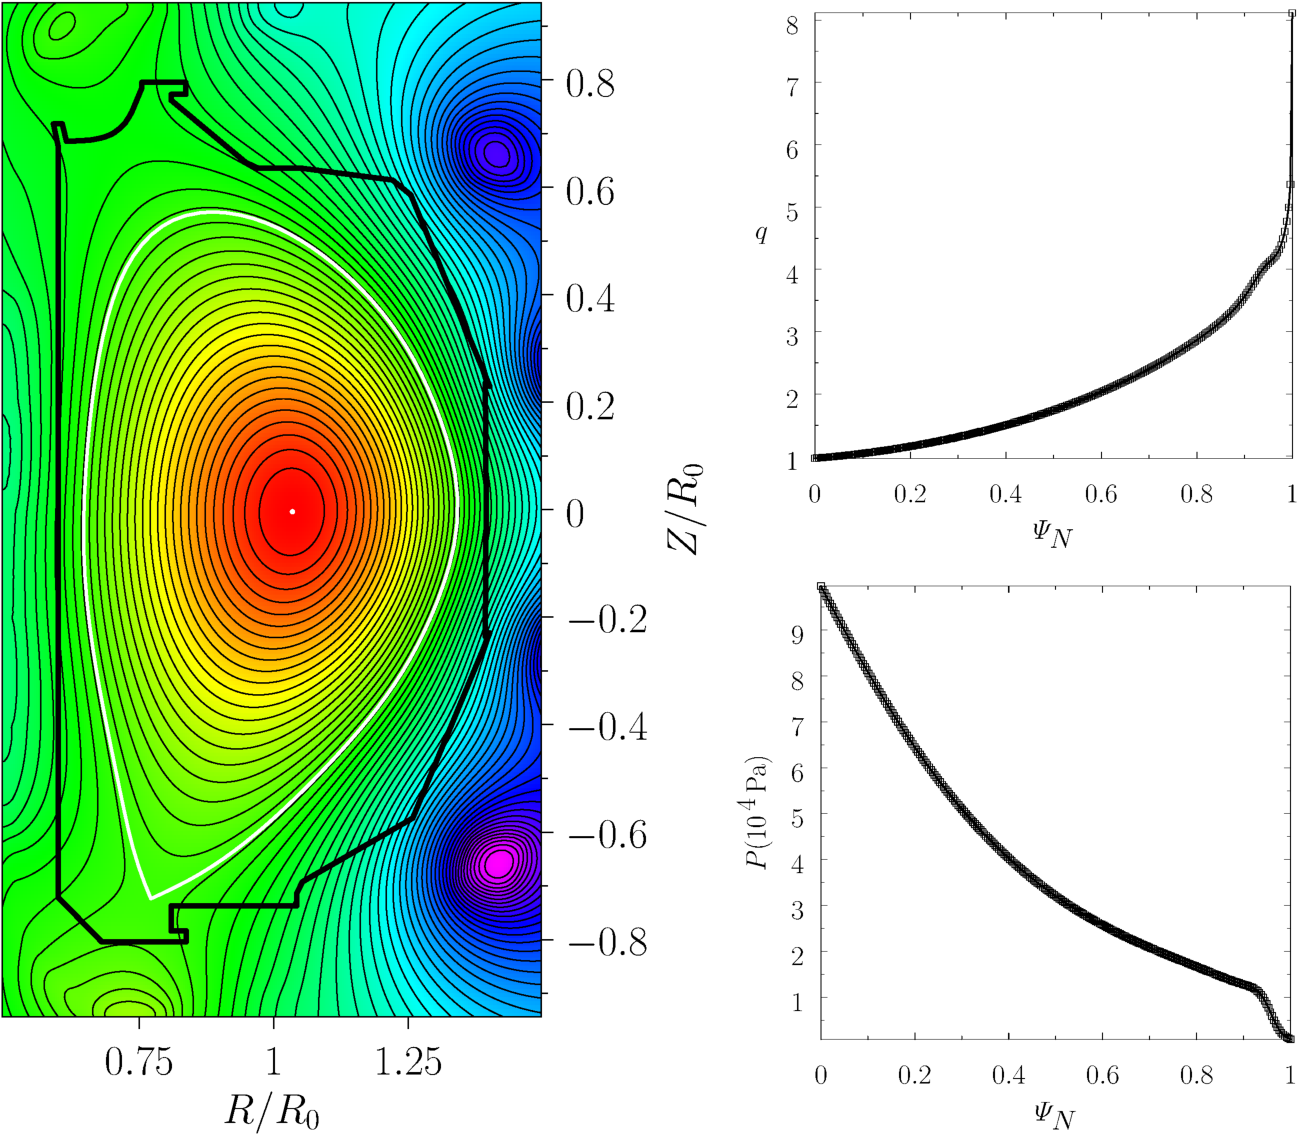
\includegraphics[height=6in]{fig2.pdf}
\caption{Composite linear/nonlinear calculation with the no-slip constraint imposed at all rational surfaces, and the natural frequencies
in the absence of the RMP determined by the local  ${\bf E}\times {\bf B}$
frequency.
Top Panel: $n=3$ natural frequencies, in absence of RMP, as functions of the least-squares linear fit to $q_{95}$ versus time
in   DIII-D discharge \#145380. Bottom Panel:  $n=3$ natural frequencies, in presence of RMP, as functions of time
in   DIII-D discharge \#145380. The red, green, blue, yellow, cyan, magenta, brown, pink,
purple, and orange  curves correspond to $m=5$, 6, 7, 8, 9, 10, 11, 12, 13, and 14, respectively. The yellow vertical bands indicate the ELM-suppression windows.} \label{fig2}
\end{figure}

\begin{figure}
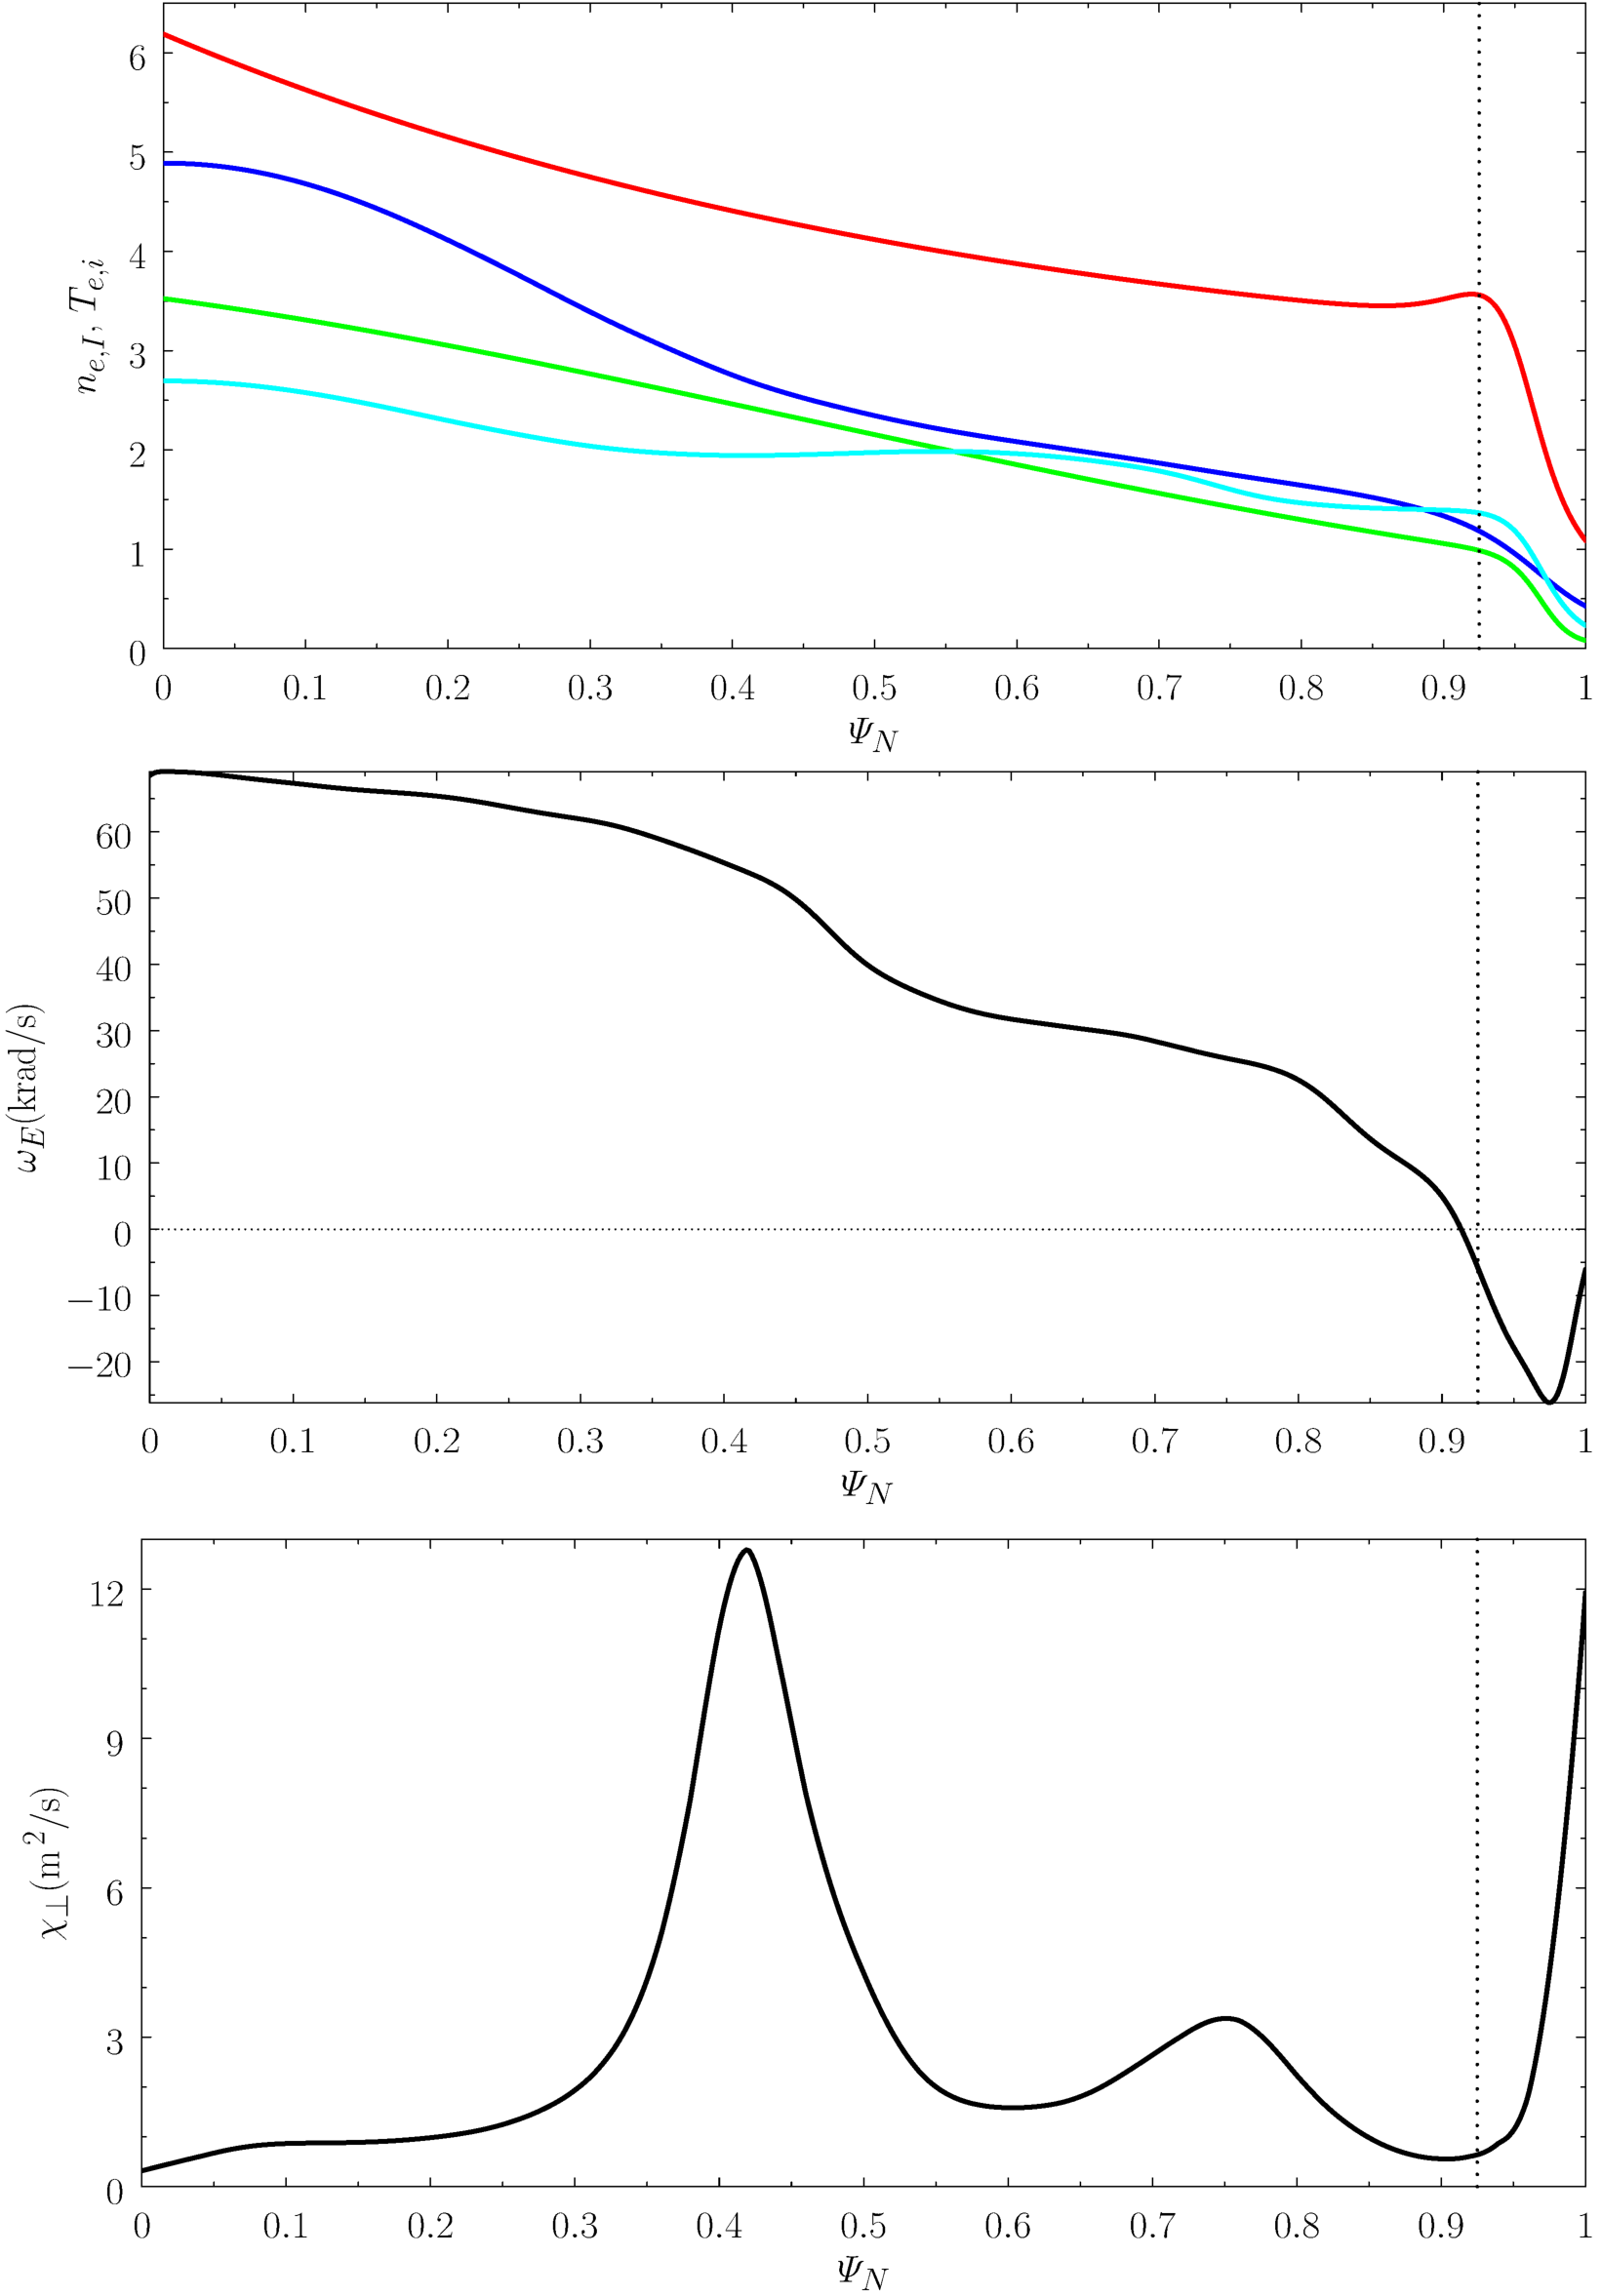
\includegraphics[height=6in]{fig3.pdf}
\caption{Composite linear/nonlinear calculation with the no-slip constraint imposed at all rational surfaces, and the natural frequencies
in the absence of the RMP determined by the local  ${\bf E}\times {\bf B}$
frequency. Top Panel: Full  $n=3$ vacuum island widths as functions of the least-squares linear fit to $q_{95}$ versus time 
in   DIII-D discharge \#145380.
Bottom Panel:  Full $n=3$ island widths as functions of time
in   DIII-D discharge \#145380. The yellow, cyan, magenta, brown, pink,
purple, and orange  areas correspond to $m=8$, 9, 10, 11, 12, 13, and 14, respectively. The yellow vertical bands indicate the ELM-suppression/mitigation windows. 
The horizontal dotted lines indicate the top of the pedestal, ${\mit\Psi}_N=0.925$.} \label{fig3}
\end{figure}

\begin{figure}
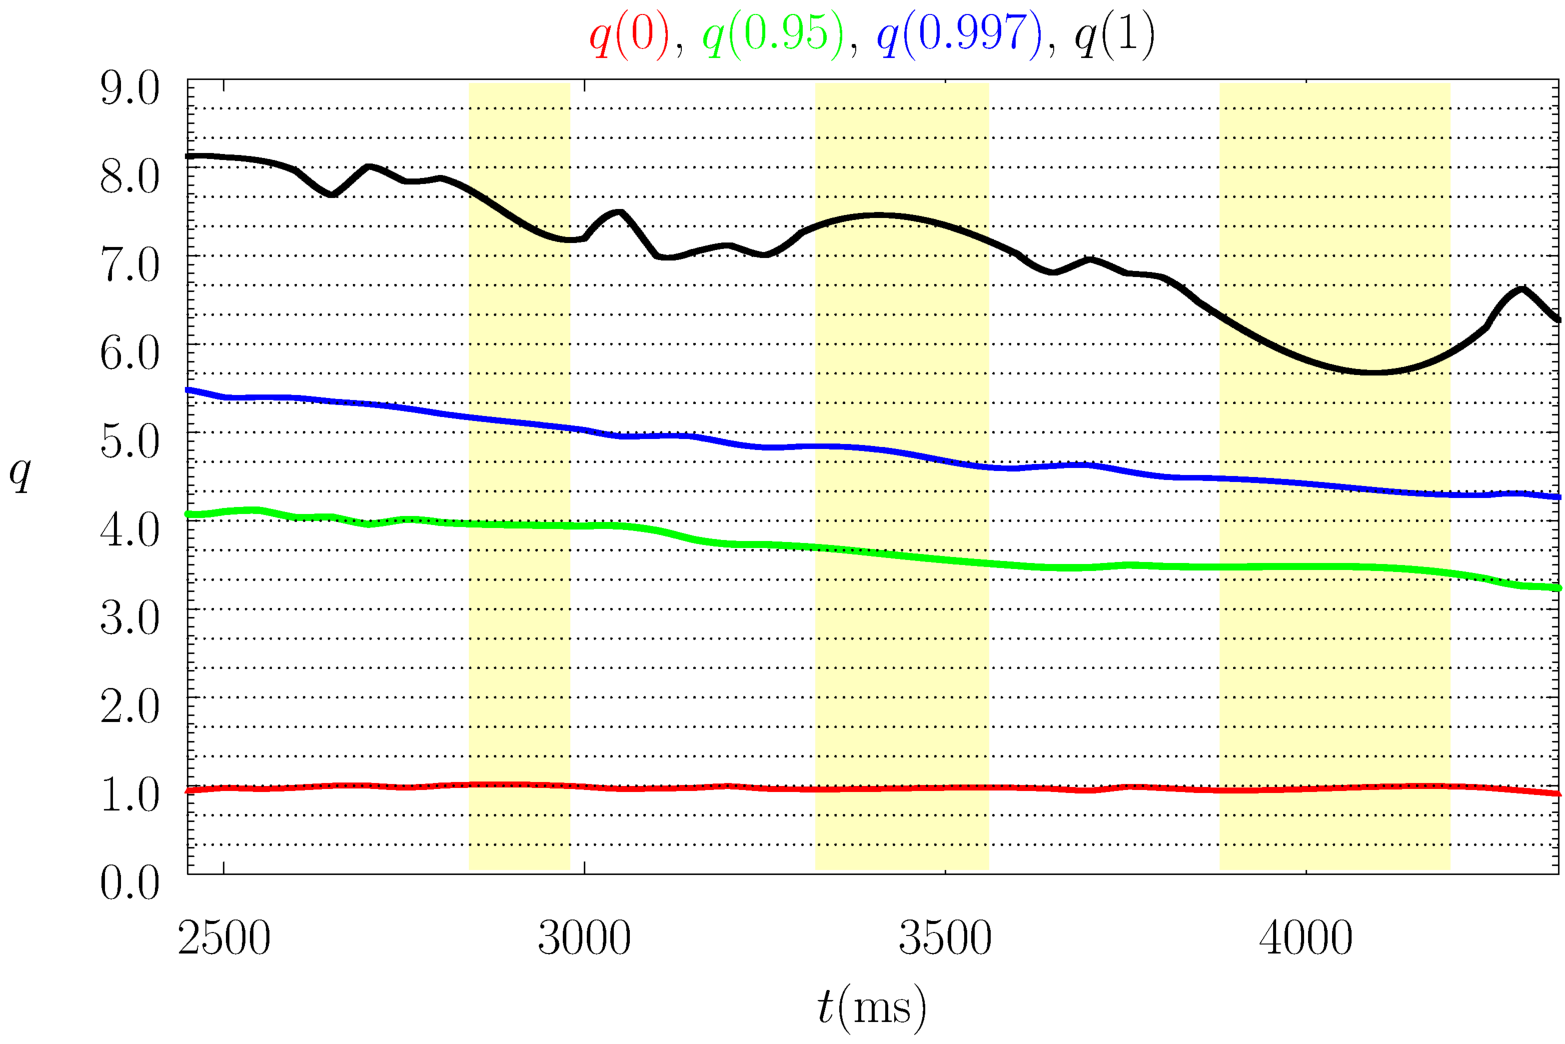
\includegraphics[height=6in]{fig4.pdf}
\caption{Composite linear/nonlinear calculation with the no-slip constraint relaxed at all rational surfaces, and the natural frequencies
in the absence of the RMP determined by the local  ${\bf E}\times {\bf B}$
frequency.
Top Panel: $n=3$ natural frequencies, in absence of RMP, as functions of the least-squares linear fit to $q_{95}$ versus time
in   DIII-D discharge \#145380.
Bottom Panel:  $n=3$ natural frequencies, in presence of RMP, as functions of time
in   DIII-D discharge \#145380. The red, green, blue, yellow, cyan, magenta, brown, pink,
purple, and orange  curves correspond to $m=5$, 6, 7, 8, 9, 10, 11, 12, 13, and 14, respectively. The yellow vertical bands indicate the ELM-suppression windows.} \label{fig4}
\end{figure}

\begin{figure}
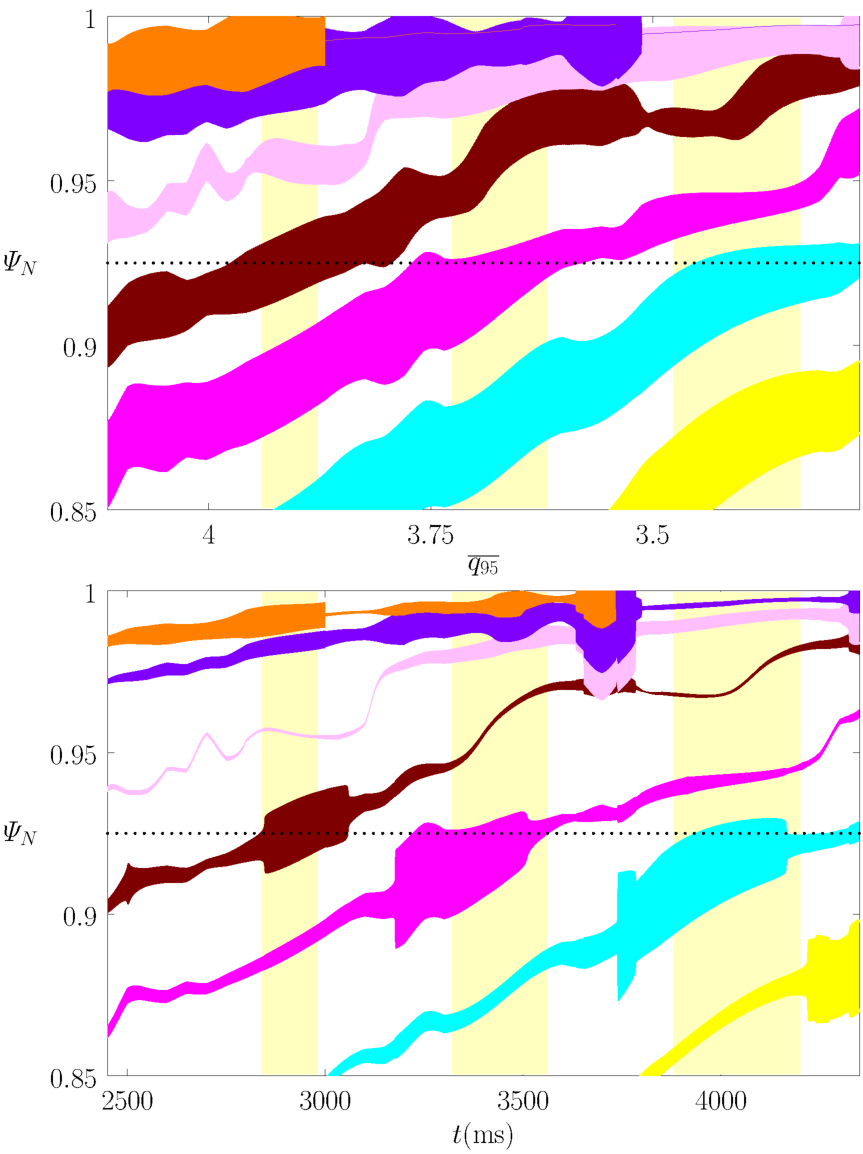
\includegraphics[height=6in]{fig5.pdf}
\caption{Composite linear/nonlinear calculation with the no-slip constraint relaxed at all rational surfaces, and the natural frequencies
in the absence of the RMP determined by the local  ${\bf E}\times {\bf B}$
frequency. Top Panel: Full  $n=3$ vacuum island widths as functions of the least-squares linear fit to $q_{95}$ versus time 
in   DIII-D discharge \#145380.
Bottom Panel:  Full $n=3$ island widths as functions of time
in   DIII-D discharge \#145380. The yellow, cyan, magenta, brown, pink,
purple, and orange  areas correspond to $m=8$, 9, 10, 11, 12, 13, and 14, respectively. The yellow vertical bands indicate the ELM-suppression/mitigation windows. 
The horizontal dotted lines indicate the top of the pedestal, ${\mit\Psi}_N=0.925$.} \label{fig5}
\end{figure}

\begin{figure}
\includegraphics[height=6in]{fig6.pdf}
\caption{Top Panel: Detail of the bottom panel of Fig.~\ref{fig2}. Bottom Panel: Detail of the bottom panel of Fig.~\ref{fig4}. } \label{fig6}
\end{figure}

\begin{figure}
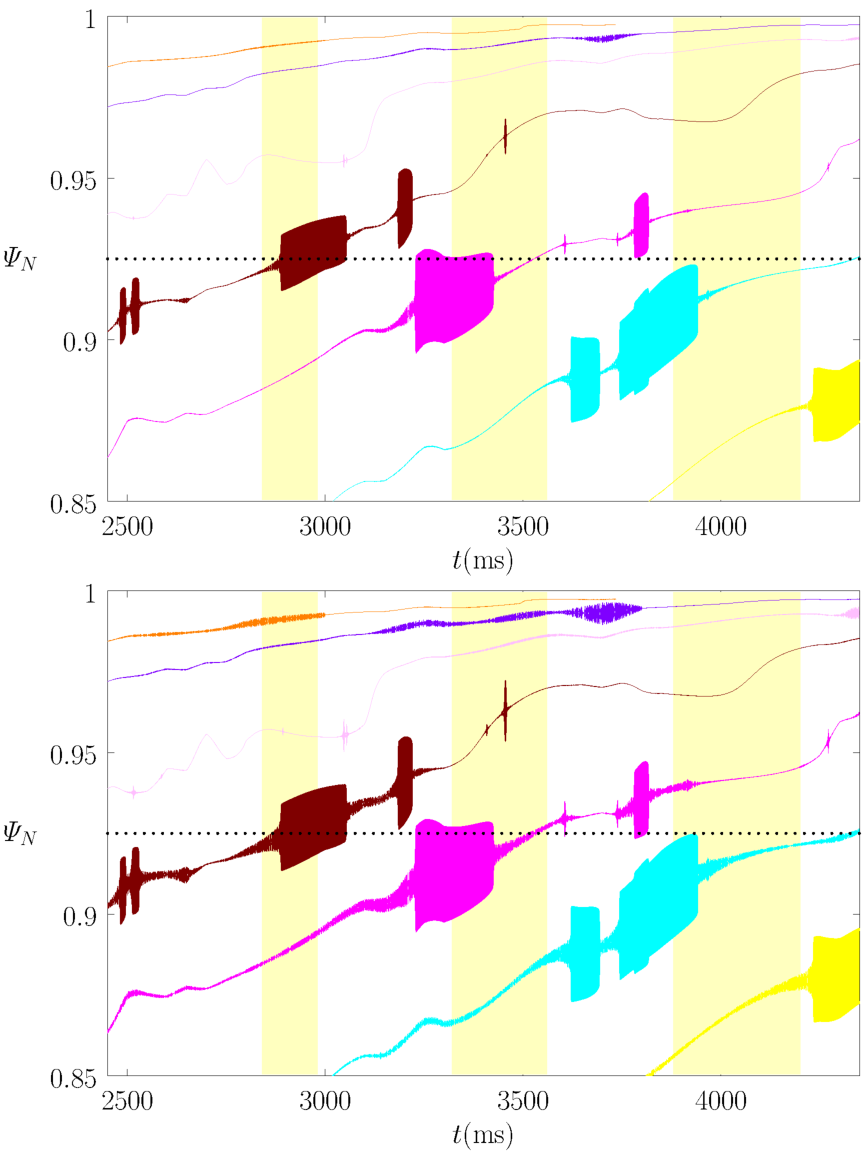
\includegraphics[height=6in]{fig7.pdf}
\caption{Linear calculation with the no-slip constraint relaxed at all rational surfaces, and  the natural frequencies
in the absence of the RMP determined by linear theory. 
 Top Panel: $n=3$ natural frequencies, in absence of RMP, as functions of the least-squares linear fit to $q_{95}$ versus time
in   DIII-D discharge \#145380.
Bottom Panel:  $n=3$ natural frequencies, in presence of RMP, as functions of time
in   DIII-D discharge \#145380. The red, green, blue, yellow, cyan, magenta, brown, pink,
purple, and orange  curves correspond to $m=5$, 6, 7, 8, 9, 10, 11, 12, 13, and 14, respectively. The yellow vertical bands indicate the ELM-suppression windows.} \label{fig7}
\end{figure}

\begin{figure}
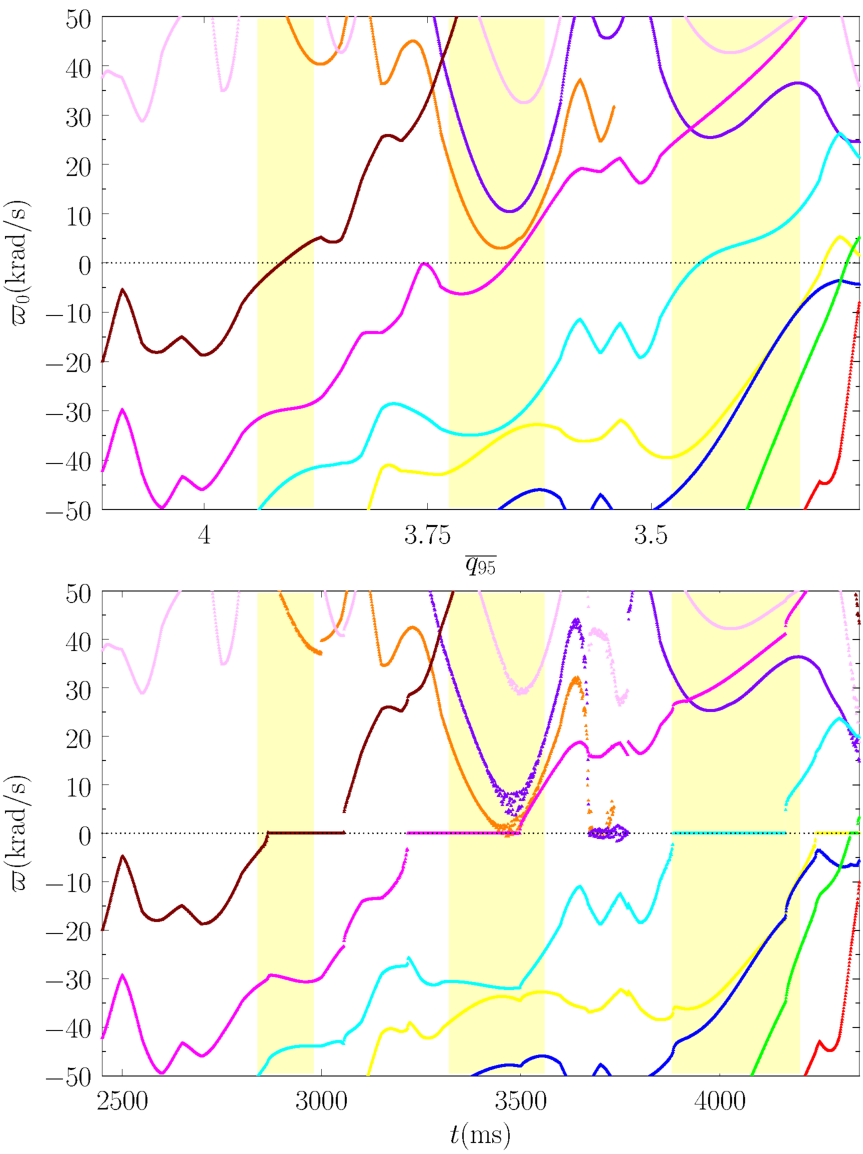
\includegraphics[height=6in]{fig8.pdf}
\caption{Linear calculation with the no-slip constraint relaxed at all rational surfaces, and  the natural frequencies
in the absence of the RMP determined by linear theory. Top Panel: Full  $n=3$ vacuum island widths as functions of the least-squares linear fit to $q_{95}$ versus time 
in   DIII-D discharge \#145380.
Bottom Panel:  Full $n=3$ island widths as functions of time
in   DIII-D discharge \#145380. The yellow, cyan, magenta, brown, pink,
purple, and orange  areas correspond to $m=8$, 9, 10, 11, 12, 13, and 14, respectively. The yellow vertical bands indicate the ELM-suppression/mitigation windows. 
The horizontal dotted lines indicate the top of the pedestal, ${\mit\Psi}_N=0.925$.} \label{fig8}
\end{figure}

\begin{figure}
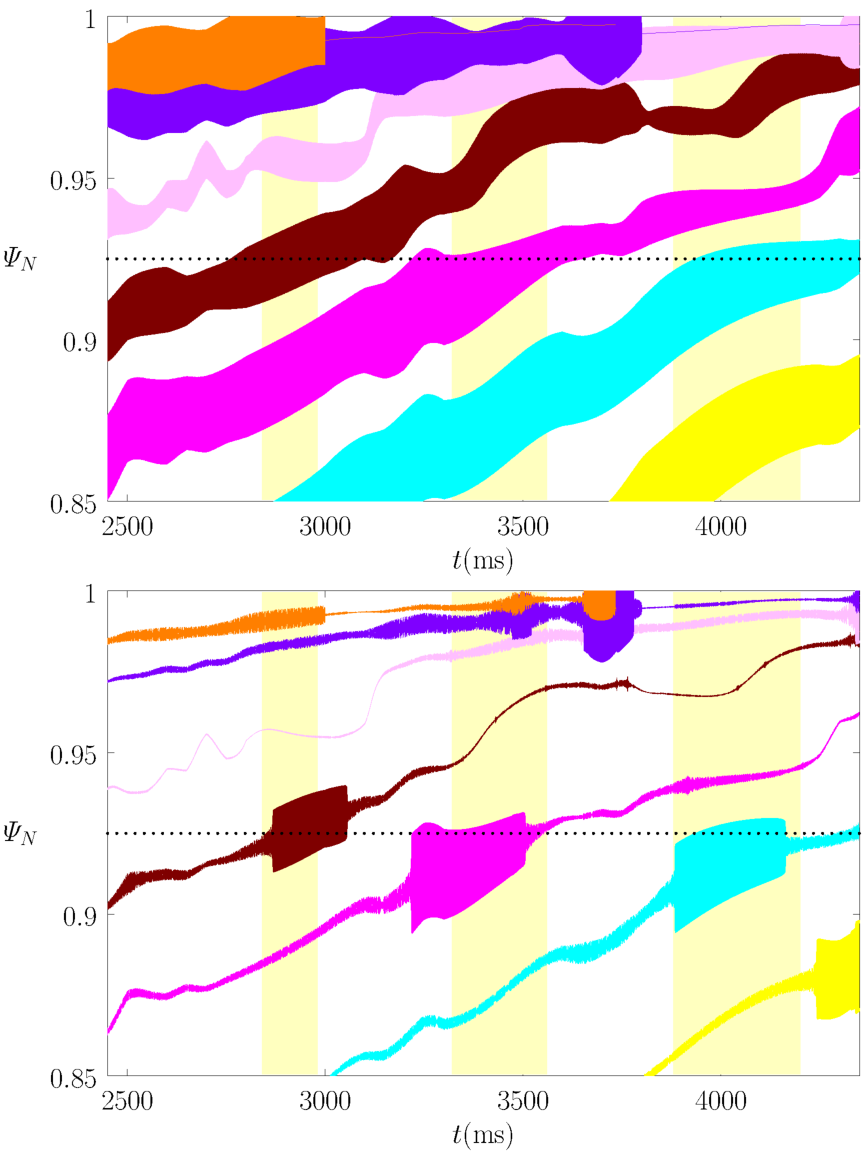
\includegraphics[height=6in]{fig9.pdf}
\caption{Composite linear/nonlinear calculation with the no-slip constraint relaxed at all rational surfaces, and  the natural frequencies
in the absence of the RMP determined by composite linear/nonlinear theory. Top Panel: $n=3$ natural frequencies, in absence of RMP, as functions of the least-squares linear fit to $q_{95}$ versus time
in   DIII-D discharge \#145380.
Bottom Panel:  $n=3$ natural frequencies, in presence of RMP, as functions of time
in   DIII-D discharge \#145380. The red, green, blue, yellow, cyan, magenta, brown, pink,
purple, and orange  curves correspond to $m=5$, 6, 7, 8, 9, 10, 11, 12, 13, and 14, respectively. The yellow vertical bands indicate the ELM-suppression windows.} \label{fig9}
\end{figure}

\begin{figure}
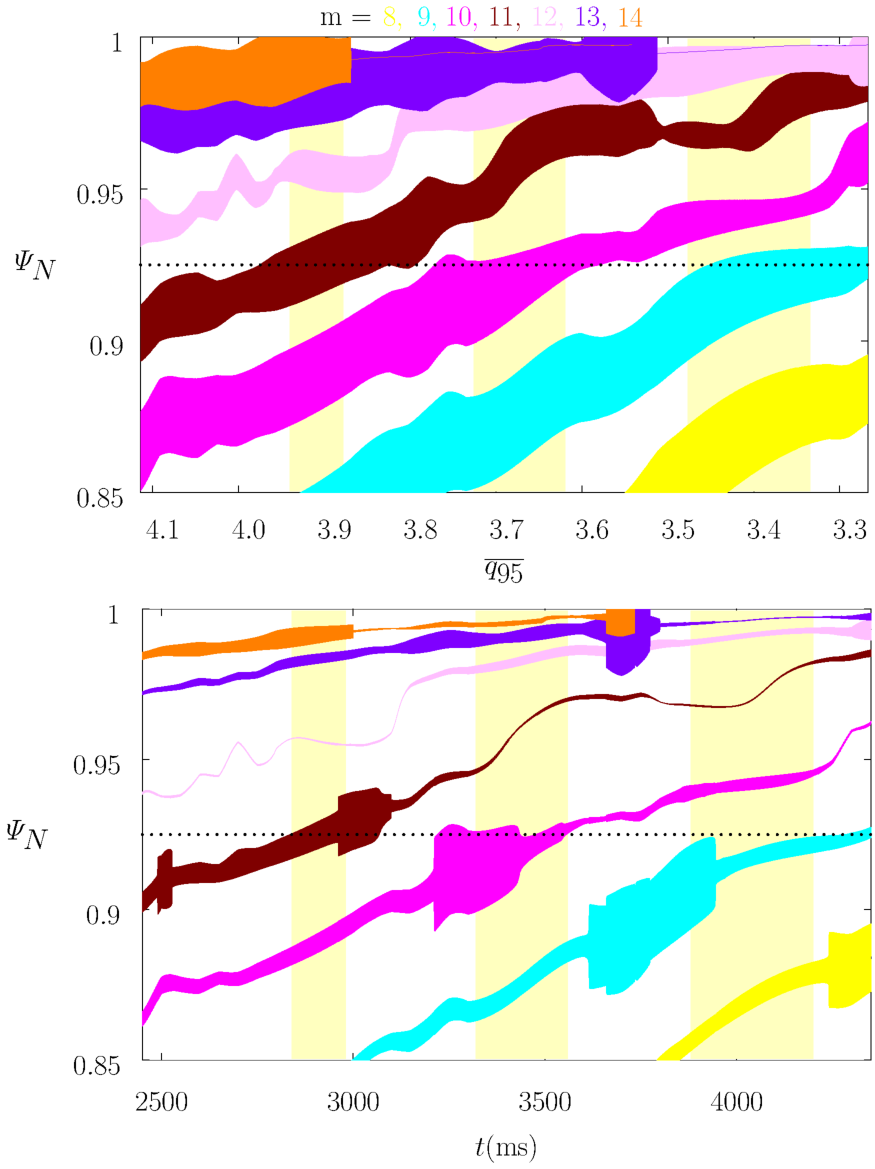
\includegraphics[height=6in]{fig10.pdf}
\caption{Composite linear/nonlinear calculation with the no-slip constraint relaxed at all rational surfaces, and  the natural frequencies
in the absence of the RMP determined by composite linear/nonlinear theory. Top Panel: Full  $n=3$ vacuum island widths as functions of the least-squares linear fit to $q_{95}$ versus time 
in   DIII-D discharge \#145380.
Bottom Panel:  Full $n=3$ island widths as functions of time
in   DIII-D discharge \#145380. The yellow, cyan, magenta, brown, pink,
purple, and orange  areas correspond to $m=8$, 9, 10, 11, 12, 13, and 14, respectively. The yellow vertical bands indicate the ELM-suppression/mitigation windows. 
The horizontal dotted lines indicate the top of the pedestal, ${\mit\Psi}_N=0.925$.} \label{fig10}
\end{figure}
\end{document}

